\section{Web information extraction}\label{sec:web_information_extraction}

Web information extraction is the process of extracting structured data from unstructured web content.
While traditionally, this was done using rule-based approaches, where developers would write specific rules to identify HTML elements via their XPath or CSS selectors, modern approaches have shifted towards machine learning and deep learning techniques.
These methods leverage the underlying structure of the webpage, such as the Document Object Model (DOM), to identify and extract relevant information.
For instance, models can be trained to recognize patterns in the DOM tree, allowing them to extract data even when the webpage layout changes, which is a common occurrence on the web.
Another requirement is for zero-shot extraction, where the model can extract information from webpages it has never seen before, without needing to be retrained for each new website.
In the context of e-commerce, web information extraction involves tasks such as extracting product details (e.g., name, price, description) from product pages, which can be challenging due to the diversity of webpage designs and the presence of boilerplate content.

\subsection{Embedded semantic metadata}\label{subsec:embedded_semantic_metadata}
More modern websites, especially those build on top of popular frameworks and content management systems, often include embedded semantic metadata in their HTML code to provide additional context about the content of the page.
This metadata is used to provide search engine crawlers and other applications with structured information about the content of the page, which can be used to improve search results and enable rich snippets in search engine results pages (SERPs).

Microdata, RDFa, and JSON-LD are common formats for embedding semantic metadata in HTML\@.

\begin{itemize}
    \item \textbf{Microdata}\cite{ronallo2012html5} is a specification for embedding structured data in HTML documents using a simple syntax.
    It allows developers to annotate their HTML with additional attributes that provide information about the content of the page.
    \item \textbf{RDFa}\cite{w3c-rdfa-primer} (Resource Description Framework in Attributes) is a W3C recommendation that provides a way to embed RDF (Resource Description Framework) data in HTML documents using attributes.
    It allows for more complex and flexible annotations compared to Microdata.
    \item \textbf{JSON-LD}\cite{w3c-json-ld11} (JavaScript Object Notation for Linked Data) is a lightweight format for encoding linked data using JSON.
    It is often used to embed structured data in web pages, and it can be easily parsed by search engines and other applications.
\end{itemize}

Most of these metadata formats are based on the Schema.org\cite{schema-org} vocabulary, which provides a standardized set of types and properties for describing various entities and their relationships on the web\@.
For example, a product page on an e-commerce website might include JSON-LD markup that describes the product's name, price, description, and availability, as shown in Listing~\ref{lst:jsonld-example}.

\begin{lstlisting}[language=json, caption={Example JSON-LD product markup from an e-commerce webpage with the Schema.org vocabulary}, label={lst:jsonld-example}, captionpos=b]
{
  "@context": "https://schema.org/",
  "@type": "Product",
  "@id": "https://lifemobile.lk/product/honor-magic-v5-5g-16gb-ram-512gb/#product",
  "name": "Honor Magic V5 5G 16GB RAM 512GB",
  "url": "https://lifemobile.lk/product/honor-magic-v5-5g-16gb-ram-512gb/",
  "description": "7.95 inches Display, 5820mAh silicon-carbon battery, Snapdragon 8 Elite, 1 Year Company Warranty",
  "image": "https://lifemobile.lk/wp-content/uploads/2025/11/Honor-Magic-V5-5G-16GB-RAM-512GB.jpg",
  "sku": "honor-magic-v5-5g-16gb-ram-512gb",
  "offers": [
    {
      "@type": "Offer",
      "priceSpecification": [
        {
          "@type": "UnitPriceSpecification",
          "price": "634285.71",
          "priceCurrency": "LKR",
          "valueAddedTaxIncluded": false,
          "validThrough": "2027-12-31"
        }
      ],
      "priceValidUntil": "2027-12-31",
      "availability": "http://schema.org/InStock",
      "url": "https://lifemobile.lk/product/honor-magic-v5-5g-16gb-ram-512gb/",
      "seller": {
        "@type": "Organization",
        "name": "Life Mobile",
        "url": "https://lifemobile.lk"
      }
    }
  ]
}
\end{lstlisting}

Of the three most common metadata formats, JSON-LD is the most widely used for embedding structured data in web pages, particularly for e-commerce websites.
An analysis of the 100 most popular e-commerce websites in the US and UK in 2023 found that only 45\% of URLs did not contain JSON-LD metadata, and 27\% contained unstructured JSON-LD metadata with errors.\cite{tierney2023structured}

Therefore, while embedded semantic metadata can be a valuable source of structured data for web information extraction, it is not universally present or consistently implemented across all websites, which can limit its effectiveness as a sole method for extracting information from the web\@.

\subsection{Vision-based approaches}\label{subsec:vision_based_approaches}
While the Document Object Model (DOM) provides a structured representation of a webpage, it can be complex and noisy, and usually fails to reflect the actual semantic grouping of content as perceived by human users.
Vision-based approaches to web information extraction address this issue by treating the webpage as an image and leveraging computer vision techniques to identify and extract relevant information.
The \textbf{Vision-based Page Segmentation (VIPS) algorithm}\cite{cai2003vips} was developed to segment a webpage into visually coherent blocks, which can then be analyzed to extract structured data.

The VIPS algorithm works by building a hierarchical tree structure of the webpage based on its visual layout, rather than its DOM structure.
Each node in the tree represents a visually coherent block of content, and the algorithm uses various visual cues such as font size, color, and spatial relationships to determine how to segment the page.

\begin{figure}[h]
    \centering
    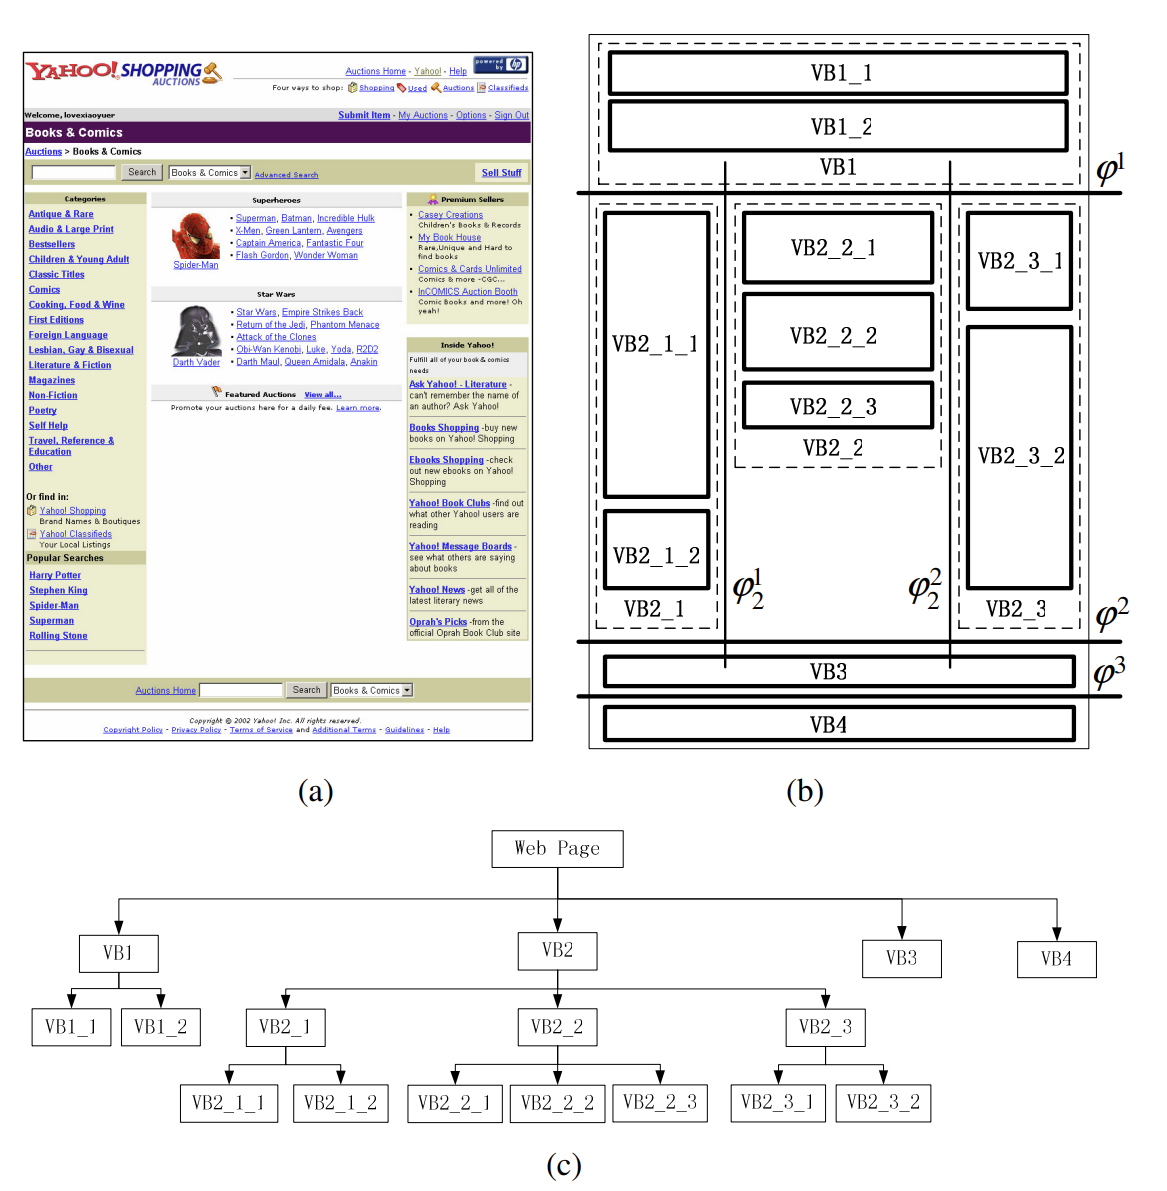
\includegraphics[width=0.8\textwidth]{images/vips}~\caption{Image segmentation of a webpage using the VIPS algorithm\cite{cai2003vips}}
    \label{fig:vips}
\end{figure}

\subsection{DOM tree node classification}\label{subsec:dom_tree_node_classification}
Another approach to web information extraction is to treat the problem as a classification task, where each node in the DOM tree is classified as either relevant or irrelevant for the information extraction task at hand.
This approach can be implemented using machine learning or deep learning models, which can learn to identify relevant nodes based on features such as the node's tag name, attributes, text content, and its position in the DOM tree.
Graph Neural Networks (GNNs) have been used to model the relationships between nodes in the DOM tree, allowing for more effective classification of relevant nodes.

ZeroShotCeres\cite{lockard2020zeroshotceres} is a model that uses a GNN to classify nodes in the DOM tree for web information extraction.
It is designed to perform zero-shot extraction, meaning it can classify nodes on webpages it has never seen before, without needing to be retrained for each new website.
The model is trained on a large dataset of webpages with labeled nodes, and it learns to generalize from this training data to classify nodes on new webpages based on their features and their relationships to other nodes in the DOM tree.

\begin{figure}[h]
    \centering
    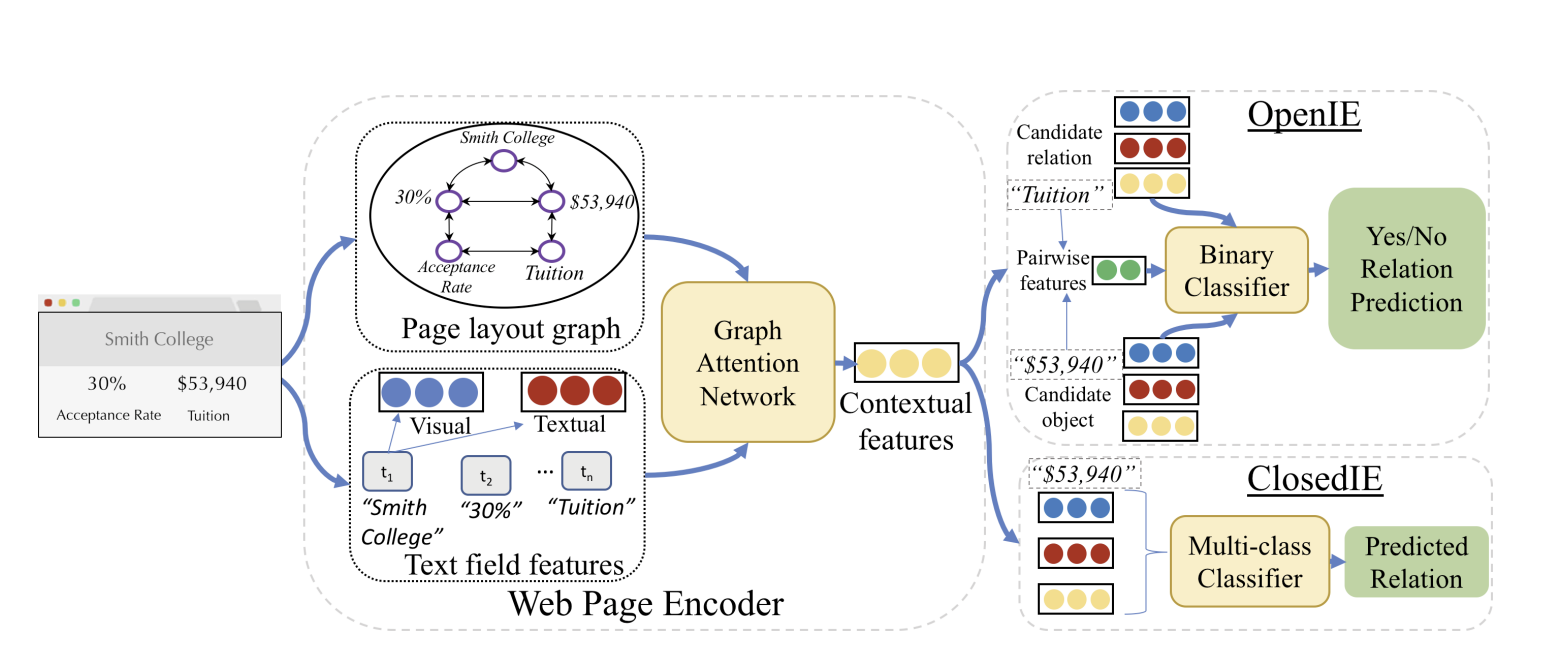
\includegraphics[width=0.8\textwidth]{images/zero_shot_ceres}~\caption{Node classification using ZeroShotCeres\cite{lockard2020zeroshotceres}}
    \label{fig:zero_shot_ceres}
\end{figure}

AttriSage\cite{potta2024attrisage} uses a similar approach to extract product attributes from e-commerce webpages by classifying nodes by treating the task as a multi-label node classification problem, where each node can be classified with multiple labels corresponding to different product attributes (e.g., name, price, description).
It uses a GNN to model the relationships between nodes in the DOM tree, allowing it to effectively classify nodes based on their features and their relationships to other nodes, even when the webpage layout varies significantly across different e-commerce websites.

\begin{figure}[h]
    \centering
    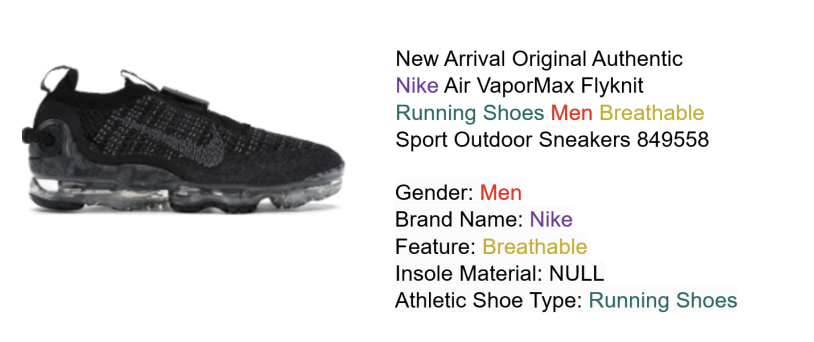
\includegraphics[width=0.8\textwidth]{images/attrisage}~\caption{Product attribute extraction\cite{potta2024attrisage}}
    \label{fig:potta2024attrisage}
\end{figure}

\subsection{Markup and layout-based approaches}\label{subsec:markup_and_layout_based_approaches}
Recent transformer architectures have been developed that integrate the structural hierarchy of HTML directly into language representations, allowing for more effective web information extraction by leveraging both the textual content and the structural layout of the webpage.
Unlike traditional models which only encode the textual content of a node, these models also encode the position of the node in the DOM tree, which can provide valuable context for understanding the relationships between different elements on the page.

\textbf{MarkupLM}\cite{li2022markuplm} encodes both the textual content of a node and its position in the DOM tree using a specialized XPath embedding layer.
It is a pretrained language model that can be fine-tuned for various web information extraction tasks.
MarkupLM also treats information extraction as a token classification task, where each token in the input sequence is classified as either relevant or irrelevant for the extraction task, allowing it to effectively identify and extract relevant information from the webpage.
Since MarkupLM does not actually render the webpage, it is very lightweight and can be used for large-scale web information extraction without the overhead of rendering webpages, while still leveraging the structural information provided by the DOM tree.

MarkupLM uses BERT architecture and is pretrained on 24 million web pages from the Common Crawl\cite{common-crawl} dataset, which allows it to learn a wide range of patterns and structures commonly found in web pages, making it effective for zero-shot extraction on new websites.

\textbf{WebFormer}\cite{wang2022webformer} is a transformer architecture that integrates the structural hierarchy of HTML directly into language representations by encoding the position of each node in the DOM tree using a specialized embedding layer.
There are three types of tokens used in WebFormer in the input layer.

\begin{itemize}
    \item \textbf{Field tokens}represent the different fields that are being extracted from the webpage, such as product name, price, description, etc.
    \item \textbf{HTML tokens} represent the HTML path of each node in the DOM tree, which provides information about the structure and layout of the webpage, allowing the model to understand the relationships between different elements on the page.
    \item \textbf{Text tokens} represent is an embedding of the textual content of each node in the DOM tree, which provides information about the content of the webpage.
\end{itemize}

WebFormer uses four specialized attention patterns (HTML-to-HTML, HTML-to-Text, Text-to-HTML, and Text-to-Text) to allow the model to effectively leverage both the structural information provided by the HTML tokens and the content information provided by the text tokens, enabling it to perform accurate web information extraction even when the webpage layout varies significantly across different websites.

\subsubsection{Performance comparison}\label{subsubsec:performance_comparison}
\begin{table}[h]
    \centering
    \begin{tabular}{llll}
        \hline
        \textbf{Benchmark} & \textbf{Metric} & \textbf{MarkupLM} & \textbf{WebFormer} \\
        \hline
        SWDE (1 seed site)  & F1    & 82.11\%           & --                 \\
        SWDE (5 seed sites) & F1    & 97.37\%           & 92.46\%            \\
        SWDE                & EM    & --                & 86.58\%            \\
        SWDE (Products)     & F1    & --                & 83.37\%            \\
        SWDE (Products)     & EM    & --                & 80.67\%            \\
        \hline
        WebSRC              & F1    & 74.47\%           & --                 \\
        WebSRC              & EM    & 68.39\%           & --                 \\
        \hline
    \end{tabular}
    \caption{Performance comparison of MarkupLM and WebFormer on standard benchmarks}
    \label{tab:markuplm-webformer-performance}
\end{table}

\subsection{Multimodal approaches}\label{subsec:multimodal_approaches}
Multimodal approaches to web information extraction leverage multiple sources of information, such as the textual content and the visual layout of the webpage, to improve the accuracy and robustness of information extraction.

LayoutLMv3\cite{huang2022layoutlmv3} is one such model that encodes text (via OCR) and layout coordinates and image patches.
It is a pretrained multimodal transformer model that can be fine-tuned for various web information extraction tasks.
LayoutLMv3 uses a combination of text, layout, and image information to perform information extraction, allowing it to effectively identify and extract relevant information from the webpage even when the layout varies significantly across different websites.
While LayoutLMv3 can achieve high accuracy on web information extraction tasks, it is computationally expensive due to the need to render the webpage and perform OCR to extract text, which can limit its scalability for large-scale web information extraction tasks.

\subsection{LLM-based approaches}\label{subsec:llm_based_approaches}
Large Language Models (LLMs) excel at zero-shot information extraction tasks, where the model can extract information from webpages it has never seen before without needing to be specifically trained.
LLMs can be prompted with the HTML content of a webpage and a specific extraction task, and they can generate structured data based on the provided input.
For example, a prompt might include the HTML content of a product page and a request to extract the product name, price, and description, and the LLM would generate a structured output containing this information.

A drawback of LLM-based approaches is that they can be computationally expensive, especially for large webpages with complex layouts, and they may not always produce accurate results, particularly when the webpage contains a lot of noise or irrelevant information.
Therefore, it is essential that the number of tokens provided as input to the LLM is limited, which can be achieved through boilerplate removal techniques that filter out irrelevant content from the webpage before feeding it into the LLM, and by converting documents into Markdown format, which can help to preserve the structural information of the webpage while reducing the amount of token introduced due to encoding HTML tags\cite{vinciguerra2026llm}.

\subsection{Summary}\label{subsec:web_info_extraction_summary}

Web information extraction approaches vary significantly in their reliance on structure, visual layout, and scale.
Rule-based methods are precise but brittle, while machine learning and transformer-based models offer greater generalisability at the cost of increased complexity.
Embedded semantic metadata provides a lightweight extraction path but is inconsistently adopted across the web.
Table~\ref{tab:web_info_extraction_summary} summarises the key approaches reviewed in this section.

\begin{table}[h]
    \centering
    \small
    \begin{tabular}{p{4cm} p{5.5cm} p{5.5cm}}
        \hline
        \textbf{Approach} & \textbf{Strengths} & \textbf{Limitations} \\
        \hline
        Embedded metadata & Structured, low overhead & Inconsistent adoption \\
        \hline
        Vision-based & Human-like layout perception & High rendering cost \\
        \hline
        DOM node classification & Structural reasoning & Complex training data \\
        \hline
        Markup \& layout & Accurate, lightweight & Complex training data \\
        \hline
        Multimodal & Robust on visually complex pages & Computationally expensive \\
        \hline
        LLM & Zero-shot, accurate, generalized & High computational cost \\
        \hline
    \end{tabular}
    \caption{Summary of web information extraction approaches}
    \label{tab:web_info_extraction_summary}
\end{table}

